\chapter{Methodik}

\section{Vorgehensmodell}

Kriterien, auf was muss geachtet werden, etc.

\section{Software}

Technologien, Plattform, etc.

\subsection{Architektur}

Abbildung~\ref{fig:position_architecture} zeigt die Position und Abbildung~\ref{fig:overview_architecture} die grobe Architektur der Software (Agile Metrics).
Die Software bildet eine Schnittstelle zwischen den einzelnen Systemen des Entwicklungsprozesses und dem System zur Darstellung der Metriken (in diesem Fall ElasticSearch und Kibana).

\begin{savenotes}
    \begin{figure}[H] 
        \centering
            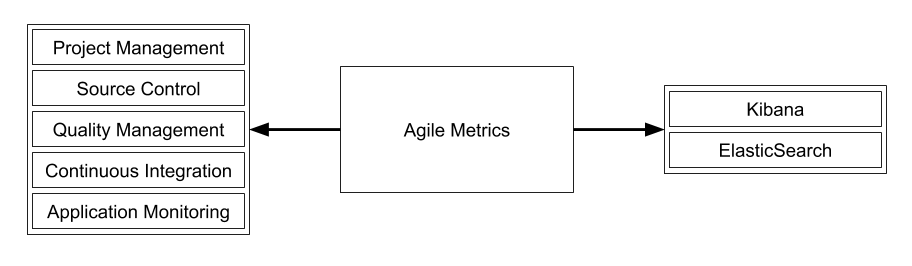
\includegraphics[width=0.8\textwidth]{img/position-overview.png}
        \caption{Position der Software}\label{fig:position_architecture}
    \end{figure}
\end{savenotes}

\begin{savenotes}
    \begin{figure}[H] 
        \centering
            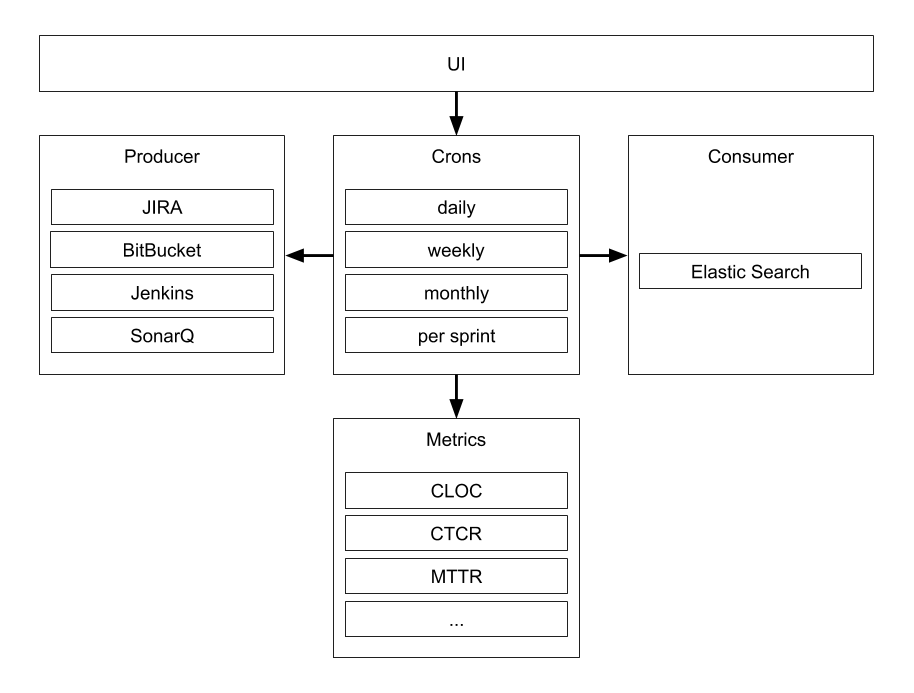
\includegraphics[width=0.8\textwidth]{img/architecture-overview.png}
        \caption{Übersicht der Software-Architektur}\label{fig:overview_architecture}
    \end{figure}
\end{savenotes}

\begin{description}
    \item[UI] \hfill \\ Bietet eine grafische Benutzeroberfläche zur Konfiguration.
    \item[Producer] \hfill \\ Sind Schnittstellen zu allen Systemen, die Messdaten erzeugen.
    \item[Crons] \hfill \\ Zeitsteuerung der Messdaten-Abfrage (z.B. täglich oder pro Sprint).
    \item[Metrics] \hfill \\ Hier können aus Messdaten direkt Metriken erstellt werden.
    \item[Consumer] \hfill \\ Sind Schnittstellen zu allen Systemen, die Messdaten und Metriken konsumieren.
\end{description}
